\documentclass[../main.tex]{subfiles}

\begin{document}
    
\chapter{Benchmark Comparison}

In this chapter we make comparison between our optimal sector universe of maximum Sharpe Ratio and benchmark sector universe. We compare each of the performance metric of both sector universes and demonstrate which sector universe has better risk-adjusted return.  

\section{Comparison Analysis}

Our benchmark sector universe is GICS S\&P 500 sectors universe. We do the backtesting of benchmark sector universe and calculate the same index we talk about in above chapters, which are cumulative ETF restructuring turnover, cumulative portfolio rebalancing turnover, portfolio return and portfolio Sharpe Ratio  respectively. The graphs of comparison between benckmark sector universe and our optimal sector unverse are: 

\begin{figure}[H]
    \centering
    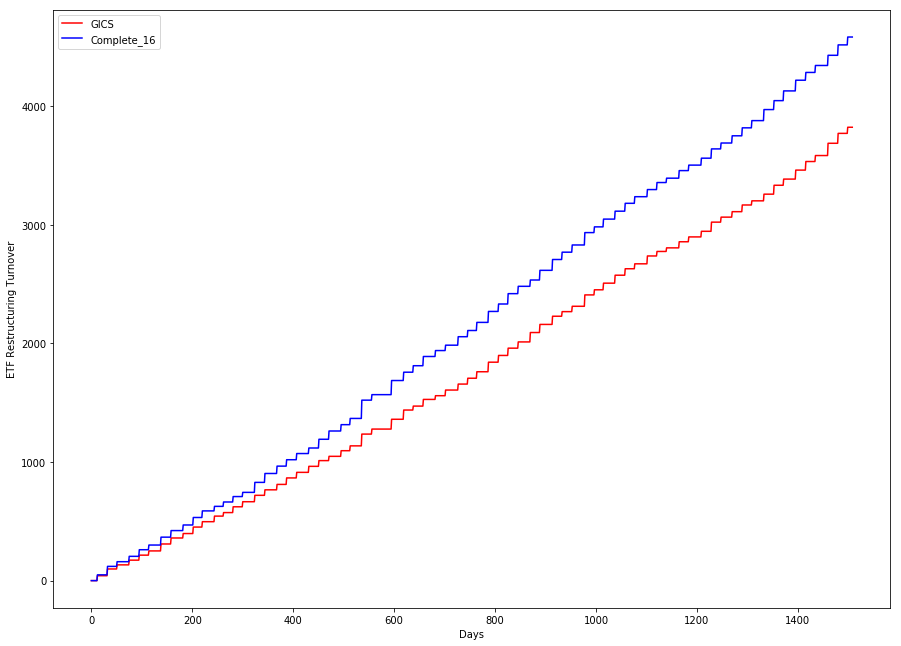
\includegraphics[scale=0.4]{images/etf_restrut_turnover_compare.png}
    \caption{Cumulative ETF Restructuring Turnover Comparison}
    \label{fig:benchmark_comparison:restrut_turnover_comparison}
\end{figure} 

\begin{figure}[H]
    \centering
    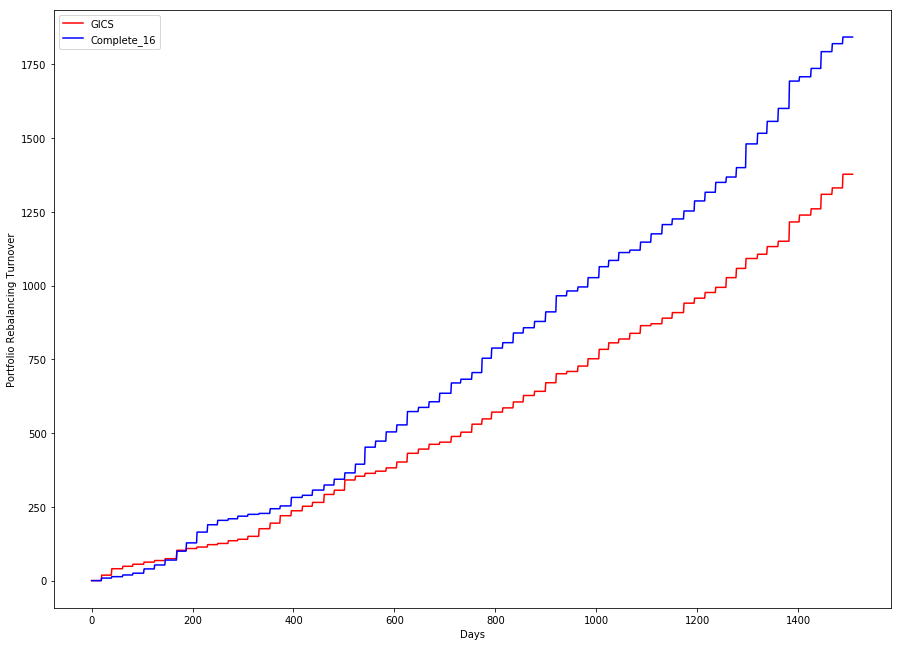
\includegraphics[scale=0.4]{images/port_rebal_turnover_compare.png}
    \caption{Cumulative Portfolio Rebalancing Turnover Comparison}
    \label{fig:benchmark_comparison:rebal_turnover_comparison}
\end{figure}

\begin{figure}[H]
    \centering
    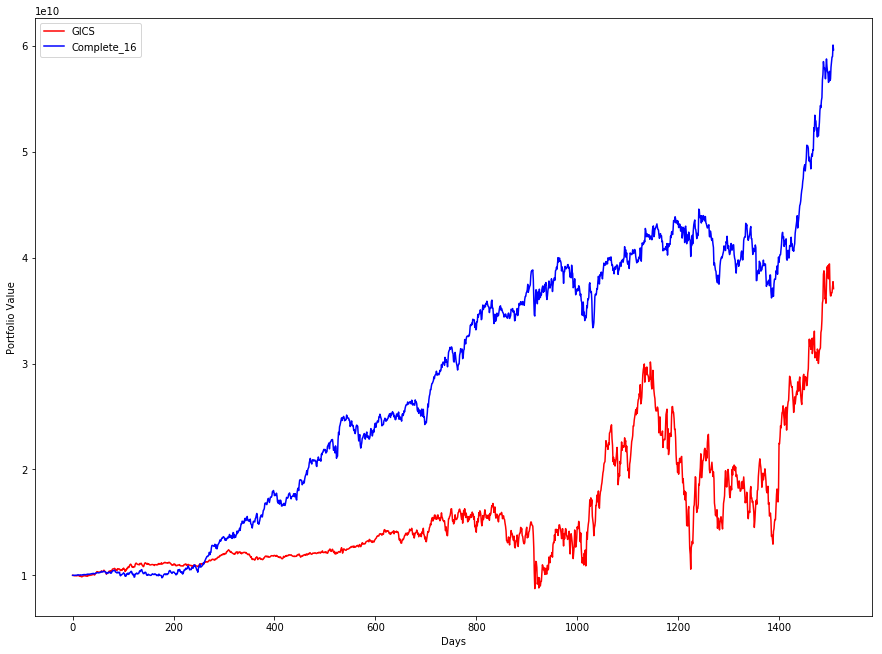
\includegraphics[scale=0.4]{images/port_value_compare.png}
    \caption{Portfolio Return Comparison}
    \label{fig:benchmark_comparison:retuern_comparison}
\end{figure}

 \begin{figure}[H]
    \centering
    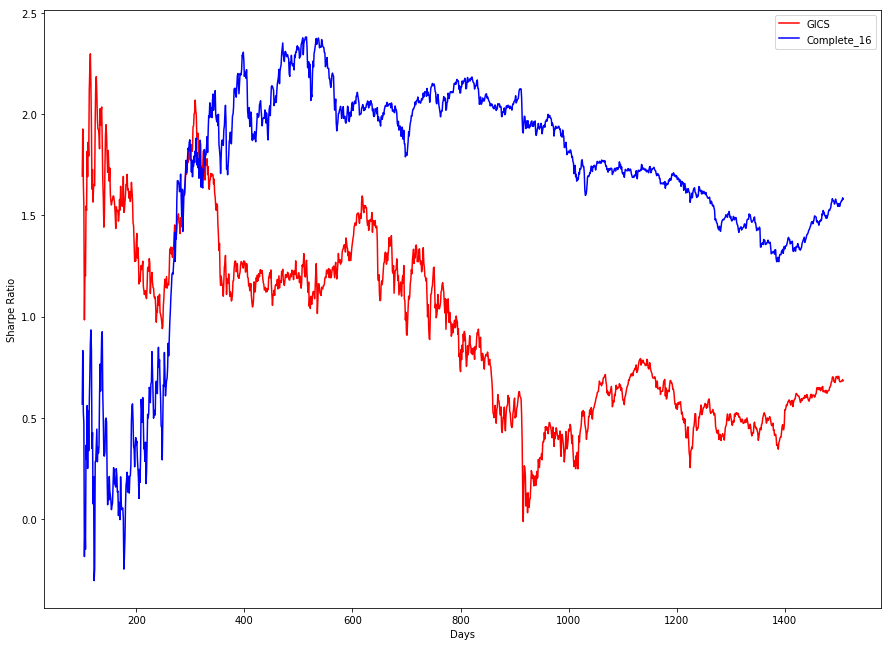
\includegraphics[scale=0.4]{images/sharpe_ratio_compare.png}
    \caption{Portfolio Sharpe Ratio Comparison}
    \label{fig:benchmark_comparison:sharpe_comparison}
\end{figure}

All red curves represent performances of benchmark sector universe and all blue curves represent performance optimal sector universe with Complete Linkage,16 Sectors. The graphs show that for cummulative turnovers,benchmark sector universe perform better than our optimal universe. One possible reason is the structure of our optimal sector. We will explore the relationship of sector structure and turnover in future work. 

Back to the topic, we highlight the comparison of Sharpe Ratio since it reflect the risk-adjusted return. From the graph, it is clear that the Sharpe Ratio of our optimal sector universe is higher than that of benchmark sector universe for most of the time during backtesting period. This indicates that our sector universe from machine-learning algorithm has hagher risk-adjusted return rhan benchmark. 

\end{document}